\documentclass[a4paper, 11pt]{article}
 
% ====== PACCHETTI NECESSARI ======
\usepackage[utf8]{inputenc}
\usepackage[T1]{fontenc}
\usepackage[italian]{babel}
\usepackage{geometry}
\usepackage{graphicx}
\usepackage[table]{xcolor}
\usepackage{tabularx}
\usepackage{array}
\usepackage{amssymb}
\usepackage{fancyhdr}
\usepackage{titlesec}
\usepackage{helvet}
\renewcommand{\familydefault}{\sfdefault}
\usepackage{lipsum}
\usepackage{hyperref}
\usepackage{booktabs}
\usepackage{enumitem}
\usepackage[utf8]{inputenc} % Specifica la codifica del file (necessaria per le accentate)
\usepackage[T1]{fontenc}    % Migliora l'output dei font per le lingue europee
\usepackage{tcolorbox}      % Per creare box colorati dei documenti
\usepackage{amsmath}   
\usepackage{longtable}      % Per formule matematiche avanzate
 
% ====== IMPOSTAZIONI GLOBALI DI STILE ======
 
% 1. DEFINIZIONE COLORI BLU-VIOLA
\definecolor{AccentColor}{RGB}{80, 90, 180} % Blu-viola principale
\definecolor{AccentLight}{RGB}{80, 90, 180} % Versione più chiara
\definecolor{AccentDark}{RGB}{50, 60, 140} % Versione più scura
\definecolor{LightGray}{RGB}{245, 245, 250}
\definecolor{MediumGray}{RGB}{200, 200, 210}
 
% --- 2. Mostra il livello 4 anche nell'Indice Es. 1.1.1.1 --- 
\setcounter{secnumdepth}{4}
\setcounter{tocdepth}{4}
 
 
% 2. IMPOSTAZIONE MARGINI
\geometry{a4paper, left=2.5cm, right=2.5cm, top=3.5cm, bottom=3.5cm}
 
% 3. STILE DEI TITOLI DI SEZIONE
\titleformat{\section}
{\normalfont\sffamily\Large\bfseries\color{AccentColor}}
{\thesection}
{1em}
{}
\titleformat{\subsection}
{\normalfont\sffamily\large\bfseries\color{AccentDark}}
{\thesubsection}
{1em}
{}
\titleformat{\subsubsection}
{\normalfont\sffamily\large\bfseries\color{AccentDark}} % Cambiare colore delle subsubsection
{\thesubsubsection}
{1em}
{}
\titleformat{\paragraph}
{\normalfont\sffamily\large\bfseries\color{AccentDark}} % Cambiare colore delle paragraph
{\theparagraph}
{1em}
{}
 
% 4. IMPOSTAZIONE HEADER E FOOTER
\pagestyle{fancy}
\fancyhf{}
\fancyhead[L]{\sffamily\bfseries\color{AccentColor}\@BYTE HOLDERS}
\fancyhead[R]{\sffamily\color{AccentColor}\thepage}
\renewcommand{\headrulewidth}{0.8pt}
\renewcommand{\headrule}{\color{AccentColor}\hrule width\headwidth height\headrulewidth \vskip-\headrulewidth}
 
% 5. IMPOSTAZIONE LINK
\hypersetup{
	colorlinks=true,
	linkcolor=AccentColor,
	urlcolor=AccentLight,
	citecolor=AccentDark,
}
 
% 6. PERSONALIZZAZIONE ELENCHI
\setlist[itemize]{itemsep=2pt, topsep=4pt}
\setlist[enumerate]{itemsep=2pt, topsep=4pt}
 
% ====== COMANDI PERSONALIZZATI ======
\makeatletter
\newcommand{\NomeGruppo}[1]{\def\@NomeGruppo{#1}}
\newcommand{\TitoloVerbale}[1]{\def\@TitoloVerbale{#1}}
\newcommand{\Sommario}[1]{\def\@Sommario{#1}}
\newcommand{\Autore}[1]{\def\@Autore{#1}}
\newcommand{\Verificatore}[1]{\def\@Verificatore{#1}}
\makeatother
 
% ====== STILE TABELLE MIGLIORATO ======
\newcolumntype{Y}{>{\raggedright\arraybackslash}X} % Colonna giustificata a sinistra
\setlength{\arrayrulewidth}{0.4pt} % Linee più sottili
\setlength{\tabcolsep}{10pt} % Spaziatura interna celle
\renewcommand{\arraystretch}{1.4} % Altezza righe
 
\newcommand{\techDef}[2]{%
	\subsubsection{#1}
	\begin{itemize}
		\item \textbf{Descrizione:} #2
	\end{itemize}
}
 
% ====== INIZIO DEL DOCUMENTO ======
\begin{document}
	
	% ====== INFORMAZIONI PER LA PAGINA DI TITOLO ======
	\NomeGruppo{BYTE HOLDERS}
	\TitoloVerbale{Norme di Progetto\textsuperscript{G}}
	\Autore{}
	\Verificatore{}
	
	\pagestyle{empty}
	
	% ====== PAGINA DI TITOLO ======
	\begin{titlepage}
		\centering
		
		
\includegraphics[width=0.55\textwidth]{../Assets/ByteHolders1.png}\par\vspace{1.5cm}
		\begin{figure}
			\centering
			\label{fig:placeholder}
		\end{figure}
		
		{\LARGE \sffamily \color{AccentColor}\bfseries Specifica Tecnica}\par
		\vspace{0.5cm}
		{\large \color{AccentColor}\sffamily }\par
		
		\vfill
		
		\noindent\color{AccentColor}\rule{\textwidth}{1pt}\par
		\vspace{0.5cm}
		
		\begin{tabularx}{0.9\textwidth}{@{}>{\bfseries\sffamily}l X@{}}
			Autore & \sffamily Alessandro Morabito, Alessandro Frison\\
			\arrayrulecolor{MediumGray}\hline \\[-1.5ex]
			Verificatore & \sffamily Alessandro Morabito \\
			\arrayrulecolor{MediumGray}\hline \\[-1.5ex] 
			Approvazione & \sffamily \\ 
			\arrayrulecolor{MediumGray}\hline 
		\end{tabularx}
		
		\vfill
	\end{titlepage}
	
	\newpage
	\section*{Registro delle versioni}
	
	\rowcolors{2}{LightGray}{white}
	\begin{longtable}{>{\centering\arraybackslash}p{1.35cm} >{\centering\arraybackslash}p{1.8cm} >{\raggedright\arraybackslash}p{2.1cm} >{\raggedright\arraybackslash}p{2.1cm} >{\raggedright\arraybackslash}p{5cm}}
		% --- Intestazione per la PRIMA pagina ---
		\rowcolor{AccentColor}
		\textcolor{white}{\textbf{Versione}} & 
		\textcolor{white}{\textbf{Data}} & 
		\multicolumn{1}{c}{\textcolor{white}{\textbf{Autore}}} & 
		\multicolumn{1}{c}{\textcolor{white}{\textbf{Verificatore}}} & 
		\multicolumn{1}{c}{\textcolor{white}{\textbf{Descrizione delle modifiche}}} \\
		\endfirsthead
		
		% --- Intestazione per le Pagine SUCCESSIVE ---
		\rowcolor{AccentColor}
		\textcolor{white}{\textbf{Versione}} & 
		\textcolor{white}{\textbf{Data}} & 
		\multicolumn{1}{c}{\textcolor{white}{\textbf{Autore}}} & 
		\multicolumn{1}{c}{\textcolor{white}{\textbf{Verificatore}}} & 
		\multicolumn{1}{c}{\textcolor{white}{\textbf{Descrizione (continua)}}} \\
		\endhead
		
		% --- Dati della tabella (Nessuna riga vuota qui in mezzo!) ---
		0.4.0 & 10/04/2026 & Alessandro Frison & & Aggiunta sezione requisiti\\
		0.3.0 & 25/03/2026 & Alessandro Frison & & Aggiunta sezione introduzione\\
		0.2.0 & 25/03/2026 & Lorenzo Grolla & Alessandro Frison & Stesura tecnologie utilizzate \\		
		0.1.0 & 24/03/2026 & Alessandro Morabito & Lorenzo Grolla & Creazione documento\\
	\end{longtable}
	\newpage
	
	
	
	% ====== INDICE ======
	\pagestyle{fancy}
	\newpage
	\tableofcontents    % Elenco dei contenuti
	\newpage
	% ====== TABELLA DI VERSIONAMENTO ======
	
	
	%\vspace{1cm}
	
	% ====== SEZIONE INFORMAZIONI INTRODUTTIVE ======
	\section{Introduzione}
	\subsection{Scopo del documento}
	Il presente documento si pone l'obiettivo di definire in modo esaustivo la \textbf{Specifica Tecnica} del progetto, fornendo una guida dettagliata alle scelte architetturali e implementative adottate. Esso rappresenta il ponte logico tra i requisiti iniziali e l'effettiva realizzazione del software, garantendo che ogni componente sia integrata in modo coerente e scalabile.

	Il documento approfondisce l'evoluzione del sistema rispetto al \textbf{Proof of Concept (PoC)} iniziale, delineando una struttura robusta e orientata alla manutenibilità a lungo termine.

	Nello specifico, questo documento si propone di:
	\begin{itemize}
		\item \textbf{Delineare l'architettura di sistema}: fornendo una panoramica delle macro-componenti e del flusso di dati tra di esse;
		\item \textbf{Dettagliare le scelte tecnologiche}: giustificando l'adozione di specifici framework, librerie e strumenti di sviluppo;
		\item \textbf{Illustrare i design pattern}: descrivendo gli schemi logici e le best practice utilizzate per risolvere problematiche ricorrenti e ottimizzare la struttura del codice;
		\item \textbf{Definire i processi di deployment}: spiegando come le diverse componenti vengono distribuite, configurate e rese operative nell'ambiente di produzione;
		\item \textbf{Fornire una base per la manutenzione}: offrendo la documentazione necessaria affinché futuri sviluppatori possano comprendere ed estendere il sistema con facilità.
	\end{itemize}
	\subsection{Glossario}
	Al fine di prevenire ambiguità e garantire una comunicazione uniforme e precisa tra i membri del gruppo e i committenti, è stato redatto un Glossario\textsuperscript{G} apposito.
	Per facilitare la lettura del presente documento, i termini tecnici o dotati di un significato specifico all'interno del dominio di progetto sono contrassegnati da una lettera «G» posta in apice (es. Parola\textsuperscript{G}).
	La definizione estesa di tali termini è reperibile nel documento citato tra i riferimenti informativi.
	\subsection{Scopo del prodotto}
	% Preso dall'AdR
	Il sistema CodeGuardian è progettato per condurre analisi approfondite sulla qualità di repository GitHub\textsuperscript{G}, garantendo un controllo rigoroso sulla gestione degli accessi e sull'autorizzazione all'avvio delle procedure di scansione. 
	\\
	La piattaforma si propone come uno strumento strategico per team di sviluppo multidisciplinari, consentendo il monitoraggio centralizzato dello stato del software e la generazione di metriche aggregate su molteplici progetti analizzati.
	
	\subsection{Riferimenti}
	\subsubsection{Riferimenti normativi}
	\begin{itemize}
		\item 
		Norme Di Progetto\textsuperscript{G} V1.1.0\\
		\url{https://byte-holders.github.io/Documentazione/RTB/Norme_Di_Progetto-V1.1.0.pdf}
		\item
		Capitolato\\
		\url{https://www.math.unipd.it/~tullio/IS-1/2025/Progetto/C2.pdf}
	\end{itemize}
	\subsubsection{Riferimenti informativi}
	\begin{itemize}
		\item
			Glossario V1.0.0\\
			\url{https://byte-holders.github.io/Documentazione/RTB/Glossario-V1.0.0.pdf}
	\end{itemize}
	
	\section{Tecnologie}
	Questa sezione descrive gli strumenti e le tecnologie adottati per lo sviluppo, il testing e il deployment del software relativo al progetto CodeGuardian. In particolare, vengono illustrati il linguaggio di programmazione, le librerie, i framework e le infrastrutture utilizzate.
 
	% =============================================
	% 2.1 LINGUAGGI DI PROGRAMMAZIONE
	% =============================================
	\subsection{Linguaggi di programmazione}
 
	\subsubsection{TypeScript}
	TypeScript è un linguaggio di programmazione open-source sviluppato da Microsoft. Si tratta di un superset di JavaScript, che introduce la tipizzazione statica, consentendo di rilevare errori di programmazione in fase di sviluppo, ridurre il numero di bug e migliorare la qualità del codice.
	\begin{itemize}
		\item \textbf{Versione:} 5.x		\item \textbf{Documentazione:} \url{https://www.typescriptlang.org/docs/}.
	\end{itemize}
	Nel contesto del progetto CodeGuardian, TypeScript è il linguaggio principale utilizzato per lo sviluppo sia del frontend che del backend. La tipizzazione statica è particolarmente utile in un progetto che coinvolge strutture dati complesse, come i report di analisi del codice e i grafi di scansione generati dall'agente AI\@.
 
	Per il frontend si utilizza TSX, un'estensione di TypeScript che permette di definire la struttura dell'interfaccia utente in modo più leggibile e dichiarativo, integrando HTML direttamente nel codice TypeScript.
 
	% =============================================
	% 2.2 FORMATO DEI DATI
	% =============================================
	\subsection{Formato dei dati}
 
	\subsubsection{JSON}
	JSON (JavaScript Object Notation) è un formato di scambio dati leggero e indipendente dal linguaggio di programmazione. È ampiamente utilizzato nello sviluppo web e nello scambio di dati tra applicazioni. JSON è basato su due strutture di dati:
	\begin{itemize}
		\item \textbf{Oggetti:} insiemi di coppie chiave-valore;
		\item \textbf{Array:} liste ordinate di valori.
	\end{itemize}
	Nel progetto CodeGuardian, JSON viene utilizzato per la trasmissione dei dati tra frontend e backend (payload delle API REST\textsuperscript{G}), per la serializzazione dei risultati di analisi, nonché per la configurazione dell'applicazione e la memorizzazione dei dati in MongoDB\@.
 
	% =============================================
	% 2.3 FRAMEWORK
	% =============================================
	\subsection{Framework}
 
	\subsubsection{NestJS}
	NestJS è un framework per Node.js\textsuperscript{G} che offre un'architettura modulare e scalabile per la creazione di applicazioni lato server. Si basa su Express.js e fornisce funzionalità aggiuntive come dependency injection\textsuperscript{G}, middleware e decorator. NestJS consente di organizzare il codice in moduli riutilizzabili e di definire facilmente controller, servizi e provider.
	\begin{itemize}
		\item \textbf{Versione:} 11.x		
		\item \textbf{Documentazione:} \url{https://docs.nestjs.com/}.
	\end{itemize}
	Nel progetto CodeGuardian, NestJS è utilizzato per creare il backend. In particolare, viene impiegato per definire i controller che gestiscono le richieste HTTP provenienti dal frontend, i servizi che implementano la business logic (gestione workspace\textsuperscript{G}, membership\textsuperscript{G}, scansioni), e i provider per l'iniezione delle dipendenze. L'architettura del backend è organizzata in sette moduli principali: \texttt{WorkspaceModule}, \texttt{MembershipModule}, \texttt{RepositoryModule}, \texttt{ScanModule}, \texttt{ReportModule}, \texttt{AnalysisModule} e \texttt{GitHubModule}.
 
	\subsubsection{LangGraph}
	LangGraph è un framework open-source per l'orchestrazione di agenti AI\textsuperscript{G}, sviluppato da LangChain Inc. Consente di modellare workflow complessi come grafi a stati, dove ogni nodo rappresenta un passo di ragionamento o un'azione, e ogni arco il flusso di controllo tra i passi. LangGraph fornisce funzionalità di gestione dello stato, checkpointing, streaming token-by-token e supporto per cicli e ramificazioni condizionali.
	\begin{itemize}
		\item \textbf{Versione:} 1.x		
		\item \textbf{Documentazione:} \url{https://langchain-ai.github.io/langgraph/}.
	\end{itemize}
	Nel progetto CodeGuardian, LangGraph è il componente centrale dell'agente di analisi del codice. Il grafo implementato definisce il flusso di scansione dei repository GitHub\textsuperscript{G}: dalla clonazione del repository, all'analisi dei file, fino alla generazione del report finale. La struttura a grafo consente di gestire ramificazioni condizionali basate sul tipo di analisi richiesta e permette di integrare verifiche intermedie e retry automatici in caso di errore.
 
	% =============================================
	% 2.4 LIBRERIE
	% =============================================
	\subsection{Librerie}
 
	% --- 2.4.1 Librerie Backend ---
	\subsubsection{Librerie backend}
 
	\paragraph{LangChain}
	LangChain è una libreria open-source che fornisce componenti riutilizzabili per l'integrazione di Large Language Model (LLM)\textsuperscript{G} in applicazioni software. Offre astrazioni per la gestione dei prompt, l'invocazione dei modelli, l'integrazione con tool esterni e la gestione della memoria conversazionale.
	\begin{itemize}
		\item \textbf{Versione:} 1.x		
		\item \textbf{Documentazione:} \url{https://js.langchain.com/docs/}.
	\end{itemize}
	Nel progetto CodeGuardian, LangChain è utilizzato in combinazione con LangGraph per la costruzione dell'agente di analisi. Fornisce le astrazioni per l'invocazione dei modelli LLM e l'integrazione con i tool di analisi del codice sorgente.
 
	\paragraph{Axios}
	Axios è un client HTTP basato su Promise per Node.js e browser. È isomorfo, cioè può essere eseguito sia nel browser che in Node.js utilizzando lo stesso codice sorgente. Lato server, Axios utilizza il modulo \texttt{http} nativo di Node.js, mentre lato client usa \texttt{XMLHttpRequest}.
	\begin{itemize}
		\item \textbf{Versione:} 1.x		
		\item \textbf{Documentazione:} \url{https://axios-http.com/docs/intro}.
	\end{itemize}
	Nel progetto CodeGuardian, Axios viene utilizzato lato frontend per effettuare richieste HTTP al backend (interrogazione delle API REST per workspace, scansioni e report) e lato backend per comunicare con servizi esterni, come le API di GitHub.
 
	\paragraph{dotenv}
	dotenv è una libreria che consente di caricare variabili d'ambiente da un file \texttt{.env} nell'oggetto \texttt{process.env} di Node.js. Permette di separare la configurazione dal codice sorgente, seguendo le best practice della metodologia Twelve-Factor App.
	\begin{itemize}
		\item \textbf{Versione:} 16.x		
		\item \textbf{Documentazione:} \url{https://github.com/motdotla/dotenv}.
	\end{itemize}
	Nel progetto CodeGuardian, dotenv è utilizzato per gestire in modo sicuro le credenziali sensibili (chiavi API dei servizi LLM, credenziali MongoDB, configurazioni AWS) sia in ambiente di sviluppo che di testing, evitando di esporre dati riservati nel codice sorgente.
 
	\paragraph{isomorphic-git}
	isomorphic-git è una reimplementazione completa di Git in puro JavaScript, compatibile sia con Node.js che con ambienti browser. Consente di eseguire operazioni Git (clone, checkout, log, status) senza dipendenze da moduli nativi C++, garantendo piena interoperabilità con l'implementazione canonica di Git.
	\begin{itemize}
		\item \textbf{Versione:} 1.x		
		\item \textbf{Documentazione:} \url{https://isomorphic-git.org/}.
	\end{itemize}
	Nel progetto CodeGuardian, isomorphic-git è una componente fondamentale del modulo \texttt{GitHubModule}. Viene utilizzato per clonare i repository GitHub degli utenti direttamente nel backend, consentendo all'agente AI di analizzare il codice sorgente localmente senza dipendere da strumenti CLI esterni. Ciò garantisce portabilità e compatibilità con ambienti containerizzati.
 
	\paragraph{Mongoose}
	Mongoose è una libreria ODM (Object Data Modeling) per MongoDB e Node.js. Fornisce una soluzione basata su schema per modellare i dati dell'applicazione, includendo validazione built-in, casting dei tipi, costruzione di query e hook per la business logic.
	\begin{itemize}
		\item \textbf{Versione:} 8.x		
		\item \textbf{Documentazione:} \url{https://mongoosejs.com/docs/}.
	\end{itemize}
	Nel progetto CodeGuardian, Mongoose è utilizzato come layer di accesso ai dati per MongoDB\@. Tutti i modelli del dominio applicativo (workspace, membership, repository, scan, report) sono definiti tramite schema Mongoose, garantendo la validazione dei dati a livello applicativo e la coerenza delle operazioni CRUD\@.
 
	% --- 2.4.2 Librerie Frontend ---
	\subsubsection{Librerie frontend}
 
	\paragraph{React}
	React è una libreria JavaScript open-source per la creazione di interfacce utente, sviluppata da Meta. Consente di definire componenti riutilizzabili che rappresentano parti dell'interfaccia, aggiornando automaticamente la vista in base allo stato dell'applicazione. React adotta un approccio dichiarativo per la definizione dell'interfaccia utente, semplificando la gestione dello stato e la sincronizzazione con il DOM\@.
	\begin{itemize}
		\item \textbf{Versione:} 19.x		
		\item \textbf{Documentazione:} \url{https://react.dev/learn}.
	\end{itemize}
	Nel progetto CodeGuardian, React è il framework di riferimento per l'interfaccia utente. La UI è organizzata in componenti funzionali che gestiscono la visualizzazione dei workspace, la lista dei repository, l'avvio delle scansioni e la consultazione dei report di analisi.
 
	\paragraph{TanStack Router}
	TanStack Router è una libreria open-source di routing type-safe per applicazioni React. A differenza di React Router, offre un sistema di routing completamente tipizzato a livello di TypeScript, con validazione dei parametri di ricerca, caricamento dati integrato e supporto nativo per search params tipizzati.
	\begin{itemize}
		\item \textbf{Versione:} 1.x		
		\item \textbf{Documentazione:} \url{https://tanstack.com/router/latest}.
	\end{itemize}
	Nel progetto CodeGuardian, TanStack Router gestisce la navigazione tra le diverse sezioni dell'applicazione: la dashboard iniziale, la vista dei workspace, le pagine di dettaglio dei repository e le schermate di visualizzazione dei report. L'integrazione type-safe con TypeScript garantisce che tutti i parametri delle rotte siano validati staticamente.
 
	\paragraph{react-markdown}
	react-markdown è una libreria React che consente di renderizzare contenuto Markdown come componenti React. Supporta la sintassi CommonMark e può essere estesa tramite plugin remark e rehype per funzionalità aggiuntive (syntax highlighting, tabelle, GFM).
	\begin{itemize}
		\item \textbf{Versione:} 9.x		
		\item \textbf{Documentazione:} \url{https://github.com/remarkjs/react-markdown}.
	\end{itemize}
	Nel progetto CodeGuardian, react-markdown viene utilizzato per visualizzare i report di analisi generati dall'agente AI, i quali sono prodotti in formato Markdown. La libreria consente di presentare all'utente il report in modo formattato, includendo intestazioni, elenchi, blocchi di codice ed eventuali tabelle riassuntive.
 
	% =============================================
	% 2.5 AUTENTICAZIONE
	% =============================================
	\subsection{Autenticazione}
 
	\subsubsection{Amazon Cognito}
	Amazon Cognito è un servizio di autenticazione e autorizzazione gestito da Amazon Web Services (AWS)\textsuperscript{G}. Consente di aggiungere funzionalità di sign-up, sign-in e gestione degli accessi alle applicazioni web e mobile. Supporta provider di identità federata (come Google e GitHub), autenticazione multi-fattore (MFA) e gestione dei token JWT\textsuperscript{G}.
	\begin{itemize}
		\item \textbf{Documentazione:} \url{https://docs.aws.amazon.com/cognito/}.
	\end{itemize}
	Nel progetto CodeGuardian, Amazon Cognito è il servizio di riferimento per la gestione dell'autenticazione degli utenti. Si occupa della registrazione, dell'accesso (anche tramite provider OAuth come GitHub), del rilascio e della verifica dei token JWT, e della gestione delle sessioni. Il backend NestJS verifica i token Cognito per proteggere le API e implementare il controllo degli accessi basato sui ruoli (owner, admin, member) all'interno dei workspace.
 
	% =============================================
	% 2.6 DATABASE
	% =============================================
	\subsection{Database}
 
	\subsubsection{MongoDB}
	MongoDB è un database NoSQL\textsuperscript{G} open-source, orientato ai documenti. A differenza dei database relazionali, MongoDB memorizza i dati in documenti flessibili in formato BSON (Binary JSON), consentendo strutture dati dinamiche che possono variare tra i documenti di una stessa collezione. MongoDB supporta query ricche, indicizzazione, aggregazioni e scalabilità orizzontale tramite sharding.
	\begin{itemize}
		\item \textbf{Documentazione:} \url{https://www.mongodb.com/docs/}.
	\end{itemize}
	Nel progetto CodeGuardian, MongoDB è il database principale dell'applicazione. Viene utilizzato per la persistenza di tutte le entità del dominio: workspace, membership, repository, scansioni e report di analisi. La natura document-oriented di MongoDB si adatta alla struttura dei report generati dall'agente AI, che possono variare in formato e complessità. L'accesso ai dati avviene tramite la libreria Mongoose.
 
	% =============================================
	% 2.7 TESTING
	% =============================================
	\subsection{Testing}
 
	\subsubsection{Jest}
	Jest è un framework di testing progettato per garantire la correttezza di qualsiasi sorgente JavaScript. Consente di scrivere test con un'API accessibile e ricca di funzionalità, che fornisce risultati rapidamente. Supporta mocking, snapshot testing, code coverage e test paralleli.
	\begin{itemize}
		\item \textbf{Versione:} 29.x		
		\item \textbf{Documentazione:} \url{https://jestjs.io/docs/getting-started}.
	\end{itemize}
	Jest è utilizzato per eseguire i test di unità e di integrazione del backend, verificando che i controller, i servizi e i moduli NestJS siano implementati correttamente. In particolare, viene impiegato per testare la logica di business dei sette moduli dell'applicazione.
 
	\subsubsection{Vitest}
	Vitest è un framework di testing per Vite. Offre funzionalità avanzate come il supporto nativo per TypeScript, la configurazione tramite file di setup e la possibilità di eseguire test in modalità watch. Questa modalità è particolarmente utile durante lo sviluppo attivo e il debugging, poiché riduce i tempi di attesa per l'esecuzione dei test.
	\begin{itemize}
		\item \textbf{Versione:} 3.x		
		\item \textbf{Documentazione:} \url{https://vitest.dev/guide/}.
	\end{itemize}
	Vitest è utilizzato per eseguire i test di unità e di integrazione del frontend, verificando che i componenti React e le funzionalità di interfaccia siano implementati correttamente.
 
	\subsubsection{Playwright}
	Playwright è un framework di testing end-to-end per applicazioni web, sviluppato da Microsoft. Consente di scrivere test in JavaScript/TypeScript, eseguirli in browser reali (Chromium, Firefox, WebKit) e verificare il comportamento dell'applicazione in modo automatizzato.
	\begin{itemize}
		\item \textbf{Versione:} 1.x		
		\item \textbf{Documentazione:} \url{https://playwright.dev/}.
	\end{itemize}
	Playwright è utilizzato per testare il frontend dell'applicazione end-to-end, verificando che i flussi utente principali (registrazione, login, creazione workspace, avvio scansione, visualizzazione report) funzionino correttamente attraverso l'intero stack applicativo.
 
	% =============================================
	% 2.8 INFRASTRUTTURA E DEPLOYMENT
	% =============================================
	\subsection{Infrastruttura e deployment}
 
	\subsubsection{Docker}
	Docker è una piattaforma open-source per lo sviluppo, la distribuzione e l'esecuzione di applicazioni in contenitori. I contenitori Docker sono unità di software che includono il codice sorgente, le dipendenze e le configurazioni necessarie per eseguire un'applicazione, garantendo ambienti consistenti e facilmente riproducibili.
	\begin{itemize}
		\item \textbf{Documentazione:} \url{https://docs.docker.com/}.
	\end{itemize}
	Nel progetto CodeGuardian, Docker è utilizzato per containerizzare i singoli servizi dell'applicazione (frontend, backend, agente AI) durante lo sviluppo e il testing locale, garantendo coerenza tra gli ambienti di sviluppo e produzione.
 
	\subsubsection{AWS Amplify}
	AWS Amplify è un servizio di hosting e deployment gestito da Amazon Web Services, progettato per applicazioni frontend e web full-stack. Supporta il deployment continuo da repository Git, la gestione automatica di certificati SSL, CDN globale e preview per le pull request.
	\begin{itemize}
		\item \textbf{Documentazione:} \url{https://docs.amplify.aws/}.
	\end{itemize}
	Nel progetto CodeGuardian, AWS Amplify è utilizzato per il deployment e l'hosting del frontend React. Fornisce un ambiente di hosting scalabile con deployment continuo collegato al repository GitHub del progetto.
 
	\subsubsection{Amazon ECS}
	Amazon Elastic Container Service (ECS) è un servizio di orchestrazione di contenitori completamente gestito da AWS\@. Consente di eseguire, fermare e gestire contenitori Docker su un cluster di istanze EC2 o tramite AWS Fargate (modalità serverless). ECS supporta la scalabilità automatica, il bilanciamento del carico e l'integrazione nativa con altri servizi AWS\@.
	\begin{itemize}
		\item \textbf{Documentazione:} \url{https://docs.aws.amazon.com/ecs/}.
	\end{itemize}
	Nel progetto CodeGuardian, Amazon ECS è utilizzato per il deployment e l'orchestrazione dei container che eseguono il backend NestJS e il servizio dell'agente AI basato su LangGraph. ECS garantisce alta disponibilità e scalabilità dei servizi backend in ambiente di produzione.
 
	\subsubsection{Amazon EC2}
	Amazon Elastic Compute Cloud (EC2) è un servizio di cloud computing che fornisce capacità computazionale ridimensionabile nel cloud AWS\@. Consente di lanciare istanze di server virtuali con diversi sistemi operativi e configurazioni hardware.
	\begin{itemize}
		\item \textbf{Documentazione:} \url{https://docs.aws.amazon.com/ec2/}.
	\end{itemize}
	Nel progetto CodeGuardian, le istanze EC2 costituiscono l'infrastruttura computazionale su cui vengono eseguiti i container gestiti da Amazon ECS\@. La scelta del tipo di istanza è calibrata in base ai requisiti di memoria e CPU necessari per l'esecuzione delle analisi AI\@.
	
	\section{Architettura}
	\subsection{Architettura di deployment}
	% Spiegazione della divisione in tre	
	\subsection{Architettura logica}
	\subsubsection{Frontend}
	\subsubsection{Backend}
	\subsubsection{Container}
\newpage
	\section{Stato dei requisiti funzionali}
	\subsection{Requisiti funzionali}
	\renewcommand{\arraystretch}{1.5}
	\rowcolors{2}{lightgray!20}{white}
	\begin{longtable}[c]{ >{\centering\arraybackslash}m{2.5cm} >{\centering\arraybackslash}m{8.3cm} >{\centering\arraybackslash}m{3.5cm} }
		\caption{Tabella dei Requisiti Funzionali} \\
		\rowcolor{AccentDark}
		\color{white}\textbf{Codice} & \color{white}\textbf{Descrizione} & \color{white}\textbf{Stato} \\
		\endhead

		R-1-F-Ob & L'utente non autenticato deve poter registrarsi al sistema inserendo username, email e password & Non completato \\
		R-2-F-Ob & Il sistema deve autenticare gli utenti tramite Amazon Cognito\textsuperscript{G} & Non completato \\
		R-3-F-Ob & Il sistema deve mostrare un messaggio di errore specifico in caso di registrazione fallita & Non completato \\
		R-4-F-De & Il sistema deve inviare un codice OTP via email per la conferma della registrazione & Non completato \\
		R-5-F-De & Il sistema deve mostrare un messaggio di errore se il codice OTP è errato o scaduto durante la conferma registrazione & Non completato \\
		R-6-F-Ob & L'utente non autenticato deve poter effettuare il login tramite username/email e password & Non completato \\
		R-7-F-Ob & Il sistema deve mostrare un messaggio di errore in caso di credenziali errate & Non completato \\
		R-8-F-Ob & L'utente deve poter recuperare la password & Non completato \\
		R-9-F-Ob & Il sistema deve mostrare un messaggio di errore in caso di ripristino password fallito & Non completato \\
		R-10-F-Ob & Il Project Manager\textsuperscript{G} deve poter invitare utenti in un workspace selezionando un ruolo & Non completato \\
		R-11-F-Ob & Il sistema deve mostrare un messaggio di errore se l'invito a un workspace non va a buon fine & Non completato \\
		R-12-F-Ob & L'utente deve poter visualizzare la lista degli inviti ricevuti con dettagli & Non completato \\
		R-13-F-Ob & Il sistema deve mostrare per ciascun invito: username mittente, username owner del workspace e nome del workspace & Non completato \\
		R-14-F-Ob & L'utente deve poter accettare o rifiutare un invito a un workspace & Non completato \\
		R-15-F-Ob & L'utente autenticato deve poter visualizzare la lista dei workspace a cui appartiene & Non completato \\
		R-16-F-Ob & Il sistema deve mostrare per ciascun workspace in lista: nome del workspace e username dell'owner & Non completato \\
		R-17-F-Ob & L'utente deve poter cercare workspace per nome & Non completato \\
		R-18-F-Ob & L'utente autenticato deve poter creare un nuovo workspace inserendone il nome & Non completato \\
		R-19-F-Ob & Il sistema deve assegnare automaticamente il ruolo di owner al creatore del workspace & Non completato \\
		R-20-F-Ob & Il sistema deve impedire la creazione di workspace con nome duplicato o non valido & Non completato \\
		R-21-F-De & L'utente deve poter visualizzare la lista dei ruoli di un workspace & Non completato \\
		R-22-F-De & Il sistema deve mostrare nome e descrizione per ciascun ruolo del workspace & Non completato \\
		R-23-F-Ob & L'utente deve poter visualizzare la lista degli utenti di un workspace & Non completato \\
		R-24-F-Ob & Il sistema deve mostrare username e ruolo per ciascun utente del workspace & Non completato \\
		R-25-F-Ob & Il Project Manager\textsuperscript{G} deve poter rimuovere un utente da un workspace & Non completato \\
		R-26-F-De & Il sistema deve verificare automaticamente lo stato di aggiornamento di una repository & Non completato \\
		R-27-F-De & Il sistema deve recuperare la data dell'ultimo push da Git\textsuperscript{G}Hub\textsuperscript{G} per verificare l'aggiornamento & Non completato \\
		R-28-F-De & Il sistema deve aggiornare lo stato della repository a 'non aggiornata' se il push è più recente della scansione & Non completato \\
		R-29-F-De & Il sistema deve gestire errori di connessione con Git\textsuperscript{G}Hub\textsuperscript{G} & Non completato \\
		R-30-F-Ob & L'utente deve poter avviare una scansione & Non completato \\
		R-31-F-Ob & Il sistema deve mostrare lo stato della scansione in corso & Non completato \\
		R-32-F-Ob & Il sistema deve notificare errori durante la scansione & Non completato \\
		R-33-F-Ob & L'utente deve poter avviare una scansione su tutte le repository di un workspace & Non completato \\
		R-34-F-Ob & L'utente deve poter avviare una scansione su una singola repository selezionando il branch\textsuperscript{G} & Non completato \\
		R-35-F-Ob & L'utente deve poter avviare una scansione su un insieme di repository selezionate & Non completato \\
		R-36-F-Ob & L'utente deve poter annullare una scansione in corso & Non completato \\
		R-37-F-Ob & Il sistema deve analizzare una o più repository & Non completato \\
		R-38-F-Ob & Architettura ad agenti coordinati da un orchestratore autocratico\textsuperscript{G} & Non completato \\
		R-39-F-Ob & Il sistema deve clonare le repository da Git\textsuperscript{G}Hub\textsuperscript{G} in locale prima dell'analisi & Non completato \\
		R-40-F-Ob & Il sistema deve distribuire l'analisi tra più componenti specializzati & Non completato \\
		R-41-F-Ob & Ciascun agente deve eseguire l'analisi di competenza e generare un report\textsuperscript{G} parziale & Non completato \\
		R-42-F-Ob & Il sistema deve aggregare i risultati & Non completato \\
		R-43-F-Ob & Il sistema deve salvare un report\textsuperscript{G} finale & Non completato \\
		R-44-F-Ob & Il sistema deve gestire URL o PAT non validi interrompendo l'operazione e notificando l'utente & Non completato \\
		R-45-F-De & L'utente deve poter visualizzare la lista dei tag\textsuperscript{G} raccolta\textsuperscript{G} di un workspace & Non completato \\
		R-46-F-De & L'utente deve poter creare un tag\textsuperscript{G} raccolta\textsuperscript{G} all'interno di un workspace & Non completato \\
		R-47-F-De & Il sistema deve impedire la creazione di tag\textsuperscript{G} raccolta\textsuperscript{G} con nome non valido o duplicato & Non completato \\
		R-48-F-De & L'utente deve poter eliminare un tag\textsuperscript{G} raccolta\textsuperscript{G} dal workspace & Non completato \\
		R-49-F-De & L'utente deve poter assegnare tag\textsuperscript{G} raccolta\textsuperscript{G} a una repository & Non completato \\
		R-50-F-De & L'utente deve poter rimuovere tag\textsuperscript{G} raccolta\textsuperscript{G} da una repository & Non completato \\
		R-51-F-Ob & L'utente deve poter visualizzare la lista delle repository del workspace & Non completato \\
		R-52-F-Ob & Il sistema deve mostrare per ciascuna repository in lista: nome, data ultima scansione, indicatore criticità, voto documentazione\textsuperscript{G}, percentuale code coverage\textsuperscript{G} & Non completato \\
		R-54-F-Ob & Il sistema deve validare il link della repository e verificare l'accesso & Non completato \\
		R-55-F-Ob & L'utente deve poter rimuovere una repository dal workspace & Non completato \\
		R-56-F-Ob & Il sistema deve permettere l'annullamento della rimozione di una repository & Non completato \\
		R-57-F-Ob & Il sistema deve avvisare l'utente se la repository da rimuovere ha scansioni in corso e richiedere conferma esplicita & Non completato \\
		R-58-F-Ob & L'utente deve poter effettuare ricerche di repository & Non completato \\
		R-59-F-De & L'utente deve poter filtrare le repository tramite barra di ricerca testuale & Non completato \\
		R-60-F-De & L'utente deve poter filtrare le repository tramite selezione di filtri multipli (linguaggio, tag, coverage, voto doc) & Non completato \\
		R-61-F-De & Il sistema deve permettere la selezione di filtri di ricerca multipli per le repository & Non completato \\
		R-62-F-De & L'utente deve poter ordinare la lista delle repository & Non completato \\
		R-63-F-Ob & L'utente deve poter visualizzare il dettaglio di una repository & Non completato \\
		R-64-F-Ob & Il sistema deve presentare la sezione completa di analisi dei test della repository & Non completato \\
		R-65-F-De & Il sistema deve mostrare la percentuale di code coverage\textsuperscript{G} & Non completato \\
		R-66-F-Ob & Il sistema deve mostrare l'elenco dei test con qualità insufficiente & Non completato \\
		R-67-F-De & Il sistema deve mostrare la percentuale di test passati & Non completato \\
		R-68-F-De & Il sistema deve mostrare l'elenco dei test non passati & Non completato \\
		R-69-F-De & Il sistema deve mostrare un messaggio informativo se nessun test è rilevato & Non completato \\
		R-70-F-Ob & Il sistema deve presentare la sezione delle informazioni tecniche (linguaggi, librerie, framework\textsuperscript{G}) & Non completato \\
		R-71-F-Ob & Il sistema deve mostrare la lista dei linguaggi rilevati & Non completato \\
		R-72-F-Ob & Il sistema deve mostrare la lista delle librerie rilevate & Non completato \\
		R-73-F-Ob & Il sistema deve mostrare la lista dei framework\textsuperscript{G} rilevati & Non completato \\
		R-74-F-Ob & Il sistema deve mostrare grafici semplificati dei risultati OWASP & Non completato \\
		R-75-F-Ob & Il sistema deve mostrare un elenco ordinato delle vulnerabilità\textsuperscript{G} OWASP & Non completato \\
		R-76-F-Ob & Il sistema deve mostrare per ciascuna vulnerabilità\textsuperscript{G}: nome/tipo, file di origine e categoria di criticità OWASP & Non completato \\
		R-77-F-De & Il sistema deve fornire i dettagli per ogni vulnerabilità\textsuperscript{G} & Non completato \\
		R-78-F-Ob & Il sistema deve presentare la sezione di analisi della documentazione\textsuperscript{G} della repository & Non completato \\
		R-79-F-Ob & Il sistema deve mostrare un voto complessivo della qualità documentale & Non completato \\
		R-80-F-De & Il sistema deve mostrare consigli per il miglioramento del README & Non completato \\
		R-81-F-Ob & Il sistema deve elencare sezioni o documenti standard mancanti & Non completato \\
		R-82-F-De & Il sistema deve mostrare suggerimenti sulla qualità del codice & Non completato \\
		R-83-F-Ob & Il sistema deve mostrare un messaggio informativo se non sono disponibili dati di scansione per una repository & Non completato \\
		R-84-F-Ob & Il sistema deve permettere la selezione del branch\textsuperscript{G} per la visualizzazione & Non completato \\
		R-85-F-Ob & Il sistema deve mostrare la lista dei branch\textsuperscript{G} disponibili per una repository & Non completato \\
		R-86-F-Ob & Il sistema deve notificare l'errore se non sono disponibili branch\textsuperscript{G} validi per una repository & Non completato \\
		R-87-F-Ob & L'utente deve poter visualizzare una visione aggregata del workspace & Non completato \\
		R-88-F-De & L'utente deve poter filtrare la visione aggregata per tag\textsuperscript{G} raccolta\textsuperscript{G} & Non completato \\
		R-89-F-Ob & Il sistema deve mostrare le metriche aggregate dei test (coverage medio, repository sopra soglia, coverage minimo) & Non completato \\
		R-90-F-Ob & Il sistema deve mostrare grafici aggregati di distribuzione linguaggi e framework\textsuperscript{G} del workspace & Non completato \\
		R-91-F-Ob & Il sistema deve mostrare percentuale repository sicure e grafico vulnerabilità\textsuperscript{G} aggregate per gravità & Non completato \\
		R-92-F-Ob & Il sistema deve mostrare voto documentazione\textsuperscript{G} minimo, medio, massimo e grafico distribuzione del workspace & Non completato \\
		R-93-F-Ob & Il sistema deve mostrare un messaggio di errore se il workspace è vuoto o senza repository nella visione aggregata & Non completato \\
		R-94-F-Ob & L'utente deve poter aggiornare le informazioni sulle repository in base all'ultima scansione & Non completato \\
		R-95-F-Op & Integrazione con CI/CD (GitHub\textsuperscript{G} Actions\textsuperscript{G}) & Non completato \\
		R-96-F-Op & Analisi storica e confronto tra versioni & Non completato \\
		R-97-F-Op & Ranking dei progetti per qualità complessiva & Non completato \\
		R-98-F-Op & Remediation interattiva con anteprima & Non completato \\
		R-99-F-Op & Notifiche integrate (Slack/Teams/Email) & Non completato \\
		R-100-F-Op & Plugin system per nuovi agenti di analisi & Non completato \\
	\end{longtable}
\newpage
	\subsection{Cruscotto riassuntivo}
	Di seguito sono riportati i grafici che mostrano lo stato di completamento dei requisiti funzionali totali, obbligatori, desiderabili e opzionali. \\
	In particolare in verde sono evidenziati i requisiti completati e in rosso quelli non completati. 
	\begin{figure}[h!]
		\centering
		
\includegraphics[width=0.35\textwidth]{../Assets/specifica_tecnica/req_totali.png}
		\caption{Percentuale di completamento dei requisiti funzionali totali}
		\label{fig:req_totali}
	\end{figure}
	\begin{figure}[h!]
		\centering
		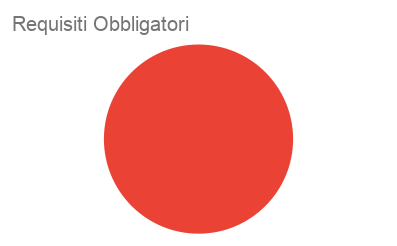
\includegraphics[width=0.35\textwidth]{../Assets/specifica_tecnica/req_obbligatori.png}
		\caption{Percentuale di completamento dei requisiti funzionali obbligatori}
		\label{fig:req_obbligatori}
	\end{figure}
	\begin{figure}[h!]
		\centering
		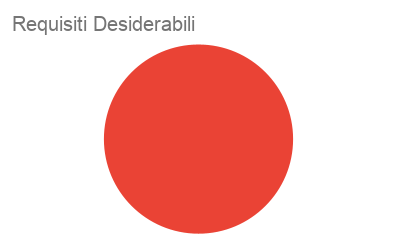
\includegraphics[width=0.35\textwidth]{../Assets/specifica_tecnica/req_desiderabili.png}
		\caption{Percentuale di completamento dei requisiti funzionali desiderabili}
		\label{fig:req_desiderabili}
	\end{figure}
	\begin{figure}[h!]
		\centering
		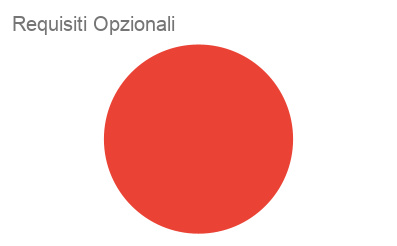
\includegraphics[width=0.35\textwidth]{../Assets/specifica_tecnica/req_opzionali.png}
		\caption{Percentuale di completamento dei requisiti funzionali opzionali}
		\label{fig:req_opzionali}
	\end{figure}

\end{document}
